\documentclass[11pt]{article}
\usepackage{amssymb,amsmath}
\usepackage{hyperref} 

\usepackage{tikz}

\usepackage[letterpaper, margin=1.0in]{geometry}


\begin{document}

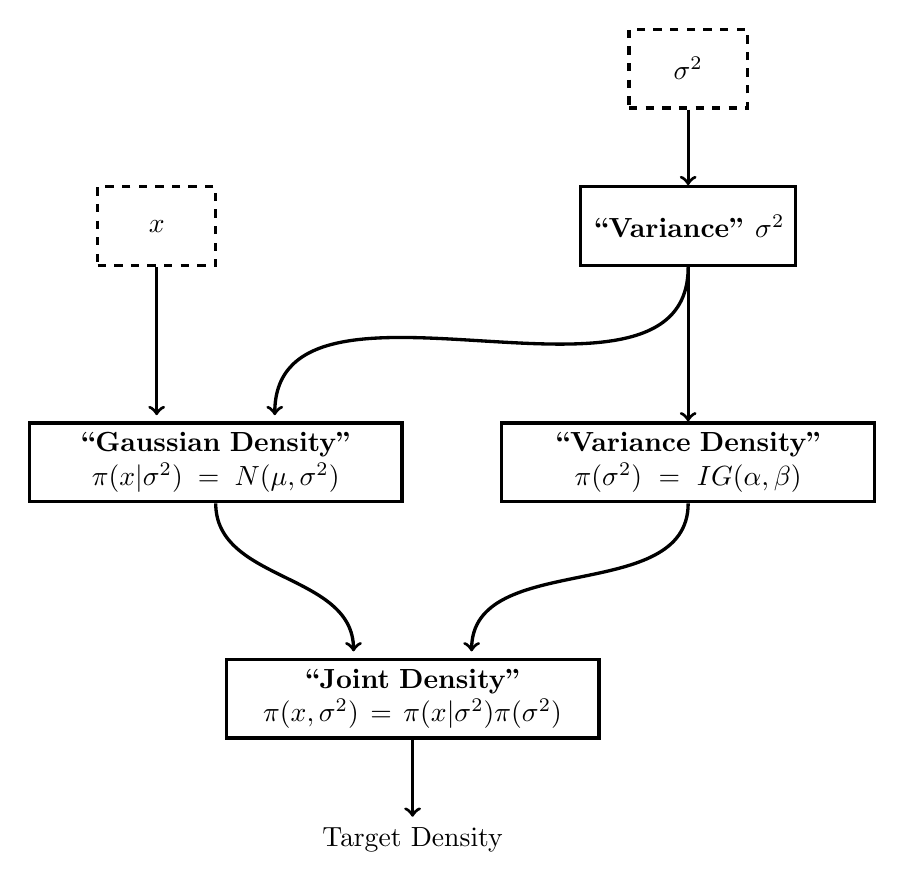
\begin{tikzpicture}[ModPiece/.style={minimum height=1cm, align=center, draw, very thick, text width=4.5cm},
ConstantPiece/.style={minimum height=1cm, align=center, minimum width=1.5cm, draw, dashed, very thick}]

\node[ConstantPiece] (x) at (-0.75,0) {$x$};
\node[ConstantPiece] (sin) at (6,2) {$\sigma^2$};

\node[ModPiece, text width=2.5cm] (s) at (6,0) {\textbf{``Variance"} $\sigma^2$};

\node[ModPiece] (xdens) at (0,-3) {\textbf{``Gaussian Density"} $\pi(x|\sigma^2) = N(\mu, \sigma^2)$};
\node[ModPiece] (sdens) at (6,-3) {\textbf{``Variance Density"} $\pi(\sigma^2) = IG(\alpha, \beta)$};

\node[ModPiece] (prod) at (2.5,-6) {\textbf{``Joint Density"} $\pi(x,\sigma^2) = \pi(x|\sigma^2)\pi(\sigma^2)$};

\draw (x.south) edge[->, very thick, out=-90, in=90] (-0.75,-2.4);
\draw (s.south) edge[->, very thick, out=-90, in=90] (0.75, -2.4);
\draw[->, very thick] (s.south) -- (sdens.north);
\draw (xdens.south) edge[->, very thick, out=-90, in=90] (1.75, -5.4);
\draw (sdens.south) edge[->, very thick, out=-90, in=90]  (3.25,-5.4);
\draw[->, very thick] (prod.south) -- (2.5,-7.5) node[below] {Target Density};
\draw[->, very thick] (sin.south) -- (s.north);

\end{tikzpicture}

\end{document}